\documentclass[12pt]{article}

%% preamble: Keep it clean; only include those you need
\usepackage{amsmath}
\usepackage[margin = 1in]{geometry}
\usepackage{graphicx}
\usepackage{booktabs}
\usepackage{natbib}

% for space filling
\usepackage{lipsum}
% highlighting hyper links
\usepackage[colorlinks=true, citecolor=blue]{hyperref}


%% meta data

\title{What is Most Popular apps in Data Analyzing}
\author{Hao Ding\\
  Department of Statistics\\
  University of Connecticut
}

\begin{document}
\maketitle

\begin{abstract}
  This is the abstract of my paper. I will provide a brief summary of my research and its key findings here.
\end{abstract}


\section{Introduction}
\label{sec:intro}

Use this section to answer three questions:
Why is the topic important/interesting?
since this topci related with our major project. 
What has been done on this topic in the literature?

What is your contribution?
Recall more person want to do this kind of things

\lipsum[1-3]

To cite a reference, here are examples.
\citet{pires2021teens} did something ... \lipsum[1]

A lot of work has been done \citep[e.g.,][]{dongarra1987computer,
}.
\lipsum[2]
Some parametric bootstrap sample size approach was proposed by
\citet{khaitovich2023most}. 


% roadmap
The rest of the paper is organized as follows.
The data will be presented in Section~\ref{sec:data}.
The methods are described in Section~\ref{sec:meth}.
The results are reported in Section~\ref{sec:resu}.
A discussion concludes in Section~\ref{sec:disc}.


\section{Data}
\label{sec:data}

Use this section to describe the data that helps to answer your research
questions. Recall Einstein's equation
\begin{equation}
  \label{eq:mc2}
  b^2 - a^2 = (b+a) * (b-a)
\end{equation}
which states that the energy $E$ of a particle in its rest frame as the product
of mass ($m$) with the speed of light squared ($c^2$).
\lipsum{1}

\section{Methods}
\label{sec:meth}

Use this section to present the methodologies that will generate results by
analyzing the data. Suppose that the radius of a circle is $r$. Then its area is
\begin{equation}
  \label{eq:area}
  a+b =ca.
\end{equation}

Equation~\eqref{eq:area} is interesting. \lipsum[1-4]

Sometimes I don't want an equation to be numbered such as this one:
\[
  f(x) = a * b /2
\]
which is the density of a standard normal variable.



\section{Results}
\label{sec:resu}

Table~\ref{tab:rv} summarizes some example draws from some distributions.
\lipsum[1-4]

\begin{table}[tbp]
  \caption{This is my first table.}
  \label{tab:rv}
\centering
\begin{tabular}{rrr}
  \toprule
Probability & value & size \\ 
  \midrule
-0.110 & 1 & 3 \\ 
  0.116 & 2 & 4 \\ 
  -0.828 & 3 & 5 \\ 
  -0.066 & 4 & 6 \\ 
  0.219 & 5 & 7 \\ 
  0.303 & 6 & 8 \\ 
  0.544 & 0 & 9 \\ 
  -2.617 & 8 & 10 \\ 
  0.747 & 1 & 11 \\ 
  -1.103 & 4 & 12 \\ 
   \bottomrule
\end{tabular}
\end{table}

Figure~\ref{fig:project} shows the distance against the speed from this dataset.


\begin{figure}[tbp]
  \centering
  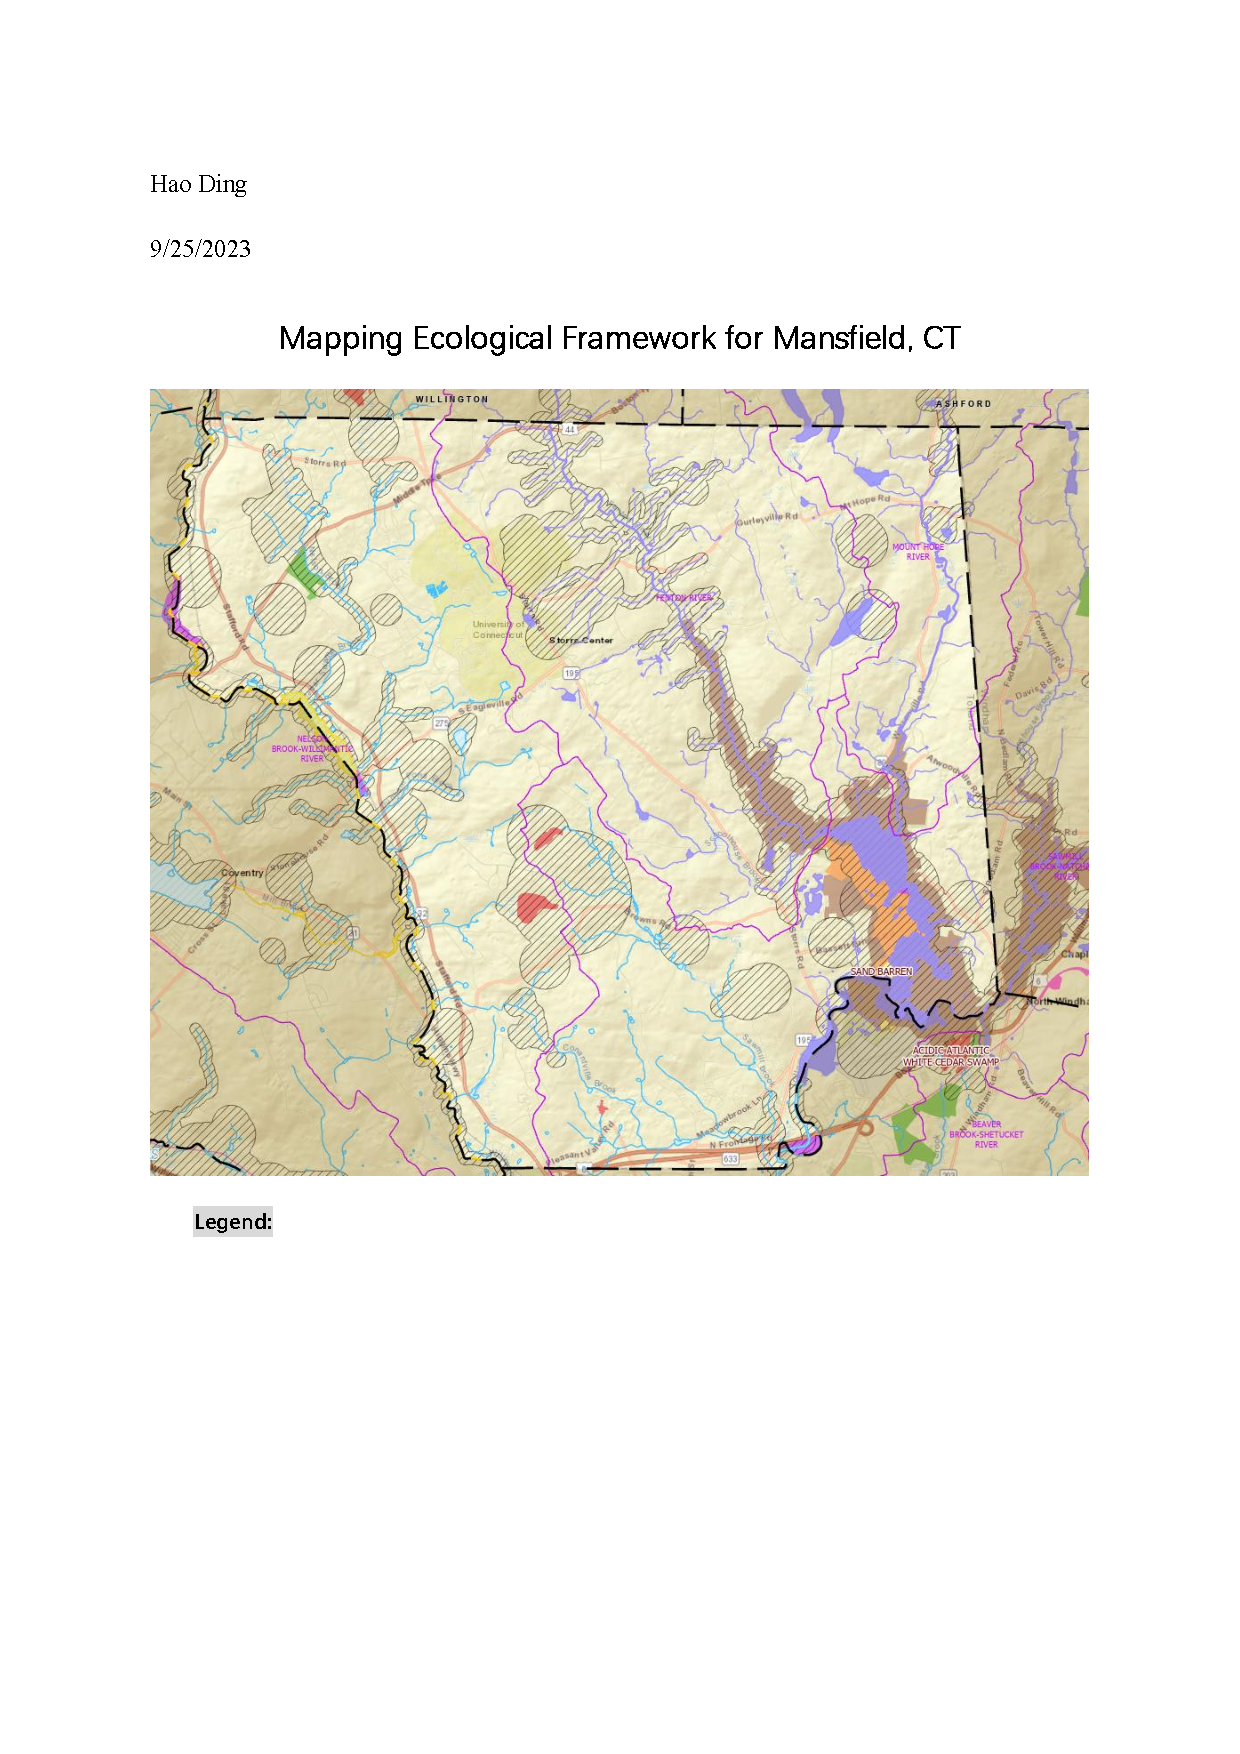
\includegraphics[width=\textwidth]{project.pdf}
  \caption{This is my first figure.}
  \label{fig:cars}
\end{figure}

\section{Discussion}
\label{sec:disc}

What are the main contributions again?
people should care about their eniveronment. 
What are the limitations of this study?
should edit the plan. 
What are worth pursuing further in the future?
sustainable development. 
\lipsum[1-2]
Watch for prevalence of diabetes \citep{dongarra1987computer}.

\bibliography{refs}
\bibliographystyle{mcap}

\end{document}